%\documentclass[12pt,a4paper]{article}
\documentclass[runningheads]{llncs}

\usepackage[latin1]{inputenc}
\usepackage{amsmath}
\usepackage{amsfonts}
\usepackage{amssymb}
\usepackage{graphicx}
\usepackage{cleveref}
\usepackage{times}
\usepackage{xspace}
\usepackage{subcaption}
\captionsetup{compatibility=false}

%%%\usepackage{authblk}
%
%%\usepackage{graphics}
%\usepackage{graphicx}
%\usepackage{hyperref}
%\usepackage{amssymb,amsmath,amstext,amsfonts}
%
%\usepackage{mathtools}
%%\DeclarePairedDelimiter\ceil{\lceil}{\rceil}
%%\DeclarePairedDelimiter\floor{\lfloor}{\rfloor}
%
%%\usepackage{a4wide}
%\usepackage[margin=2.5cm,nohead]{geometry}
%
%\usepackage{fullpage}
%\usepackage{amsfonts,amsmath,amssymb,amsthm,boxedminipage,color,url,fullpage}
%\usepackage{enumerate,paralist}
%\usepackage[numbers]{natbib} % \citet{foo} -> Foo et al. [5]
%%\usepackage[dvipdfm,pdfstartview=FitH,colorlinks,linkcolor=blue,filecolor=blue,citecolor=blue,urlcolor=blue]{hyperref} % blue links
%\usepackage[labelfont=bf]{caption}
%\usepackage{aliascnt,cleveref}
%
%
%\usepackage{breqn}
%
%\usepackage{epic,eepic}
%\usepackage{array}
%
%\usepackage{graphicx}
%\usepackage{caption}
%\usepackage{subcaption}
%
%\usepackage{xspace}


% % % for comments
\usepackage{todonotes}
\newcommand{\am}[1]{\todo[color=green!50!white]{\scriptsize Aka: #1}} 
\newcommand{\pp}[1]{\todo[color=blue!40!white]{\scriptsize Pao: #1}} 
\newcommand{\mm}[1]{\todo[color=red!40!white]{\scriptsize Mat: #1}} 
%%%%%%%%%%%%%%%%%


%%% comment in LNCS %%%%%
%\newtheorem{lemma}{Lemma}[section]
%\newtheorem{proposition}[lemma]{Proposition}
%\newtheorem{conjecture}[lemma]{Conjecture}
%\newtheorem{theorem}[lemma]{Theorem}
%\newtheorem{corollary}[lemma]{Corollary}
\newtheorem{observation}[lemma]{Observation}
%\newtheorem{claim}[lemma]{Claim}
\newtheorem{assumption}[lemma]{Assumption}

%\theoremstyle{definition}
%\newtheorem{definition}[lemma]{Definition}
%\newtheorem{example}[lemma]{Example}

%\theoremstyle{remark}
%\newtheorem{remark}[lemma]{Remark}
%\newtheorem{notation}[lemma]{Notation}

%%% end comment in LNCS %%%%%%

%\hypersetup{colorlinks=true,linkcolor=blue,citecolor=blue,filecolor=blue,urlcolor=blue}


\providecommand{\keywords}[1]{\textbf{\text{Keywords:}} #1}

\definecolor{emphcol}{gray}{.75}
\newcommand{\take}[1]{\colorbox{emphcol}{$#1$}}

%\newcommand{\SPoA}{SPoA}
\renewcommand{\epsilon}{\varepsilon}



%%% PoA and PoS definitions %%
\newcommand{\PoA}{\textbf{PoA}\xspace}
\newcommand{\SPoA}{\textbf{SPoA}\xspace}
\newcommand{\PoS}{\textbf{PoS}\xspace}
\newcommand{\SPoS}{\textbf{SPoS}\xspace}
\newcommand{\aSPoS}{\textbf{adaptive SPoS}\xspace}




\begin{document}


\title{\bf Sequential Solutions in Machine Scheduling Games}  

%

%%%% comment in LNCS style %%%
%\author[1]{Paul Giessler}
%\author[2]{Akaki Mamageishvili}
%\author[1]{Mat\'u\v{s} Mihal\'ak}
%\author[2]{Paolo Penna}


%\affil[1]{Department of Data Science and Knowledge Engineering, Maastricht University, Netherlands}
%\affil[2]{Department of Computer Science, ETH Zurich, Switzerland}

\date{}
%%%%% end comment in LNCS %%%

\author{Paul Giessler\inst{1} \and Akaki Mamageishvili\inst{2} \and Mat\'u\v{s} Mihal\'ak\inst{1} \and Paolo Penna\inst{2}}
\institute{Department of Data Science and Knowledge Engineering, Maastricht University, Netherlands}
\institute{Department of Computer Science, ETH Zurich, Switzerland}

\maketitle





\begin{abstract}
	We consider the classical machine scheduling, where $n$ jobs need to be scheduled on $m$ machines, with the goal of minimizing the makespan, i.e., the maximum load of any machine in the schedule.
	%
	We study inefficiency of schedules that are obtained when jobs arrive sequentially one by one, and choose themselves the machine on which they will be scheduled. Every job is only interested to be on a machine with a small load (and does not care about the loads of other machines). Every job knows the behavior and incentives of other jobs, and knows the order in which the jobs make the decision. 
	%
	In game theory, the described setting forms an \emph{extensive-form game}, and the resulting schedules are known as \emph{subgame-perfect equilibria}. 
	
	We measure the inefficiency of a schedule as the ratio of the makespan obtained in the worst-case equilibrium schedule, and of the optimum makespan. This ratio is known as the \emph{sequential price of anarchy (SPoA)}. 
	%
	We also introduce alternative inefficiency measures, which allow for a favorable choice of the order in which the jobs make their decisions.
	%we call a (adaptive) sequential price of stability, which we define as the best-case price of anarchy taken over all permutations of the jobs in which they make decisions.
	%
	We first disprove the conjecture of Hassin and Yovel (OR Letters, 2015) claiming that for unrelated machines, i.e., for the setting where every job can have a different processing time on every machine, the sequential price of anarchy for $m=2$ machines is at most 3. 
	%
	We provide an answer for the setting with $m=2$ and show that the sequential price of anarchy grows at least linearly with the number $n$ of players, i.e., $SPoA = \Omega(n)$.
	%
	Furthermore, we show that for a certain order of the jobs, the resulting makespan is at most linearly larger than the optimum makespan.
	%
	To the end, we show that if an authority can change the order of the jobs adaptively to the decisions made by the jobs so far (but cannot influence the decisions of the jobs), then there exists an adaptive ordering in which the jobs end up in an optimum schedule.
	%
%	
%In this paper we study inefficiency of solutions obtained by sequential players in machine scheduling, both the cases of unrelated and identical machines.  In \cite{Hassin} authors conjectured that sequential price of anarchy for $2$ unrelated machines is at most $3$. We disprove this conjecture by providing an example which shows that sequential price of anarchy grows linearly in the number of players. On the other hand, imposing a little restriction on the sequence of agent arrival we can show that they can achieve at most linearly worse makespan compared to optimum. Moreover, if some authority has a full power on the sequence of player arrival, but does not restrict players to act selfishly after fixing the order, they can achieve optimum solution. To the end we consider the case of identical machines and construct matching lower bound examples to sequential price of anarchy. 
\end{abstract}

%%%%%%%%%%%%%%%%%%%%%%%%%%%%%%%%%%%%%%%%%%%%%%%%%%%%%%%%%%%%%%%%%%%%%%%%%%%%%%%%
%%%   Introduction
%%%%%%%%%%%%%%%%%%%%%%%%%%%%%%%%%%%%%%%%%%%%%%%%%%%%%%%%%%%%%%%%%%%%%%%%%%%%%%%%
%
\section{Introduction}\label{sec:intro}

Machine scheduling is a classical and fundamental optimization problem. There is an enormous literature in the scientific world about machine scheduling, see, e.g., the textbook by Pinedo~\cite{Pinedo/2012} and the survey by Chen, Potts, and Woeginger~\cite{Chen+Potts+Woeginger/1999} for the fundamental results and further references.

We consider the classical problem of scheduling $n$ jobs on $m$ \emph{unrelated} machines. In this problem, each job has a (possibly different) processing time on each of the $m$ machines, and a feasible schedule is simply an assignment of jobs to machines. For any such schedule, the load of a machine is the sum of all processing times of the jobs assigned to that machine. In this optimization problem, the objective is to find a schedule minimizing the
\emph{makespan}, that is, the maximum load among the machines. 

This problem has been also studied from a \emph{game theoretic} prospective where jobs correspond to players who \emph{selfishly} aim at minimizing their own cost, and choose which machine to place their own job accordingly. This leads to some \emph{equilibrium} in which no player has an incentive to deviate, though the resulting schedule may not necessarily be optimal  in terms of makespan. The so-called \emph{price of anarchy} \cite{PoAoriginal} quantifies the efficiancy loss due to such selfish behavior by comparing the social cost of the worst equilibrium with the optimal social cost. In particular, they do so by considering the social cost as the makespan of the resulting schedule and by restricting to the case of \emph{identical} machines.

Such an equilibrium will have some \emph{social cost}, that is, the makespan of the corresponding schedule.\footnote{When each player chooses deterministically one machine, this definition is obvious. When equilibria are \emph{mixed} or randomized, each player chooses one machine according to some probability distribution, and the social cost is the expected makespan of the resulting schedule.} The \emph{price of anarchy}, introduced by Koutsoupias and Papadimitriou~\cite{PoAoriginal}, is a standard way to quantify the (in)efficiency of equilibria, and it is defined as the worst case ratio of the makespan of an equilibrium schedule over the makespan of a social optimum. 
%
A slightly more optimistic measure of the efficiency of equilibrium schedules is the \emph{price of stability}~\cite{PoSoriginal}, defined as the best case ratio of the makespan of an equilibrium schedule over the makespan of a social schedule.

 
Such an equilibrium will have some \emph{social cost}, that is, the makespan of the corresponding schedule.\footnote{When each player chooses deterministically one machine, this definition is obvious. When equilibria are \emph{mixed} or randomized, each player chooses one machine according to some probability distribution, and the social cost is the expected makespan of the resulting schedule.} The \emph{price of anarchy}, introduced by Koutsoupias and Papadimitriou~\cite{PoAoriginal}, is a standard way to quantify the (in)efficiency of equilibria, and it is defined as the worst case ratio of the makespan of an equilibrium schedule over the makespan of a social optimum. 
%
A slightly more optimistic measure of the efficiency of equilibrium schedules is the \emph{price of stability}~\cite{PoSoriginal}, defined as the best case ratio of the makespan of an equilibrium schedule over the makespan of a social schedule.

 
%
%In general, the processing time of a job can be different on each of the machines. In this case we talk about \emph{unrelated} machines. In the more restricted case of \emph{identical} machines, jobs can have different processing times, but each job has the same processing time on every machine.
%

Much of the previous research has considered the algorithmic problem of finding a schedule of the minimum makespan.
%
Only recently, this scheduling setting was considered from a game theoretic perspective. There are two main approaches: in the first approach, machines are viewed as players, while in the second approach, the jobs are viewed as players. 
%
In this paper we consider the latter case. 
%
%Machines in general are unrelated, meaning that for each job %different machines may need different times to execute this job. %In case of identical machines, we assume that jobs may have %different weights but machines are identical, meaning that each %job needs the same time on all machines. 
%
Every job is owned by a player. Every player decides the machine on which the job will be processed. 
%
Every player aims to minimize her cost, which is equal to the load of the machine to which it assigns her job.
%

In game theory, the result of the players' decisions is an equilibrium schedule, i.e., a schedule in which no player regrets her decision (choice of a machine). 
%
Since every player is only interested in the load of the machine containing her job, an equilibrium schedule may not minimize the makespan, which is also called the \emph{social cost} in game theory. 
%
It is thus an interesting question to quantify the efficiency of equilibrium schedules, compared to a \emph{social optimum}, which is a schedule minimizing the social cost (makespan).

%The social cost of an assignment is the maximum load among all %the machines, also called makespan. Ideally we want to minimize %the social cost, which is called social optimum. That is, we aim %to find an assignemt of players to machines which minimizes the %maximum load over the machines. Since players only care about %their costs, this goal is not always achieved. 

\emph{Price of anarchy}, introduced by Koutsoupias and Papadimitriou~\cite{PoAoriginal}, is a standard way to quantify the (in)efficiency of equilibrium schedules, and is defined as the worst case ratio of the makespan of an equilibrium schedule over the makespan of a social schedule.
%
A slightly more optimistic measure of the efficiency of equilibrium schedules is the \emph{price of stability}~\cite{PoSoriginal}, defined as the best case ratio of the makespan of an equilibrium schedule over the makespan of a social schedule.
%

Typically, in the literature, simultaneous games are considered, i.e., settings in which all players take their decisions at the same time in the beginning of the game. 
%
This approach is debatable, because in some real situations, players do not make their decisions necessarily at the same time. Even more, in some settings, players arrive one by one, and thus make their decisions sequentially.
%

In this paper, we study exactly the setting when players arrive one by one, and make their decision at the moment they arrive, knowing the order of the players in which they arrived and will arrive, and knowing the decisions of the previous players.
%
All players have the same goal (having the job on a machine with small load), and players are aware of others' goal.
%
In such a setting, the rational agents end up in an equilibrium schedule known as the \emph{subgame perfect Nash equilibrium}.
%

The efficiency of solutions obtained in this sequential setting was first studied in \cite{originalSPOA}. Initial results showed that naturally defined \emph{sequential price of anarchy} is at most $m\cdot 2^n$, while it is at least $n$. Later, the upper bound has been slightly improved to $2^n$, and the lower bound considerably to $2^{O(\sqrt{n})}$~ \cite{bilo}. 
%
Hassin and Yovel~\cite{Hassin} studied the case of identical machines, and by establishing a connection to the schedules obtained by the greedy algorithm of Graham~\cite{Graham} proved an upper bound of $2-\frac{1}{m}$ for the sequential price of anarchy, while for a restricted version of a sequential price of anarchy, where agents are sorted by decreasing their processing times, Hassin and Yovel \cite{Hassin} proved an upper bound of $\frac{4}{3}-\frac{1}{3m}$.

The sequential price of anarchy has been studied in few other settings as well. See \cite{originalSPOA} and \cite{SPOAcongestion} for other examples.

\subsection{Our contributions}\label{sec:contributions}

Our work is motivated by the following conjecture made by Hassin and Yovel \cite{Hassin}: 
\begin{quote}
	\emph{The \SPoA for  $m=2$ unrelated machines and any number of players is $3$.}
\end{quote}
We disprove this conjecture by showing a lower bound where the sequential price of anarchy grows \emph{linearly in the number of players $n$}. 
%
The result is also interesting in the sense that there is no upper bound on the sequential price of anarchy as a function of the number of machines $m$. 
%
On the other hand, if the initial order can be fixed by some authority, efficient schedules can be achieved. 
%
In particular, we show that a large class of sequences result in a schedule which is at most linear factor worse than the optimum.
%
Moreover, if we assume that there is an authority that has a full control of the order in which the players make their decisions,  in particular, if it does not only fix the initial sequence but can change the sequence adaptively depending on the choices of previous players, then the players can achieve an optimum schedule for the case $m=2$.
%
We complement this result with a negative example which shows that even for $m=3$ machines obtaining optimum solution is impossible even with an adaptive order of players. 

%One of the most important directions in algorithmic game theory is to find the efficiency of Nash equilibria solutions. The worst case ratio of a Nash equilibrium solution over the optimum solution is called price of anarchy, introduced in \cite{PoAoriginal}, while the best case ratio is called price of stability, \cite{PoSoriginal}. In both cases, simultaneous games are considered. It is assumed that all players take their decisions at the same time in the beginning of the game. This assumption is debatable, because in many of the real occasions players arrive one by one. Further assumptions we make are that players enter the game once and stay till the end, and also they get a decision only when they arrive. All the players in the game are rational, they have full knowledge on the following players after them and thay also know that the others are all rational. The efficiency of solution obtained based on these assumptions in machine scheduling game was first studied in \cite{originalSPOA}. Initial results showed that sequential price of anarchy given $m$ machines and $n$ players is at most $m\cdot 2^n$, while it is at least $n$. Later, in \cite{bilo} authors improved the upper bound slightly to $2^n$ and the lower bound considerably to $2^{O(\sqrt{n})}$. 
%
%Authors in \cite{Hassin} studied the case of identical machines and by establishing connection to the greedy best response solutions from \cite{Graham} proved upper bound of $2-\frac{1}{m}$ for sequential price of anarchy, while for a restricted version of sequential price of anarchy, where agents are sorted by decreasing their weights, authors in \cite{Hassin} proved an upper bound $\frac{4}{3}-\frac{1}{3m}$.
%
%Some other games have also been studied in the context of sequential price of anarchy, for the examples see \cite{originalSPOA} and \cite{SPOAcongestion}.
%
%\subsection{Our contributions}\label{sec:contributions}
%
%This paper was motivated by the conjecture of the authors of \cite{Hassin}. They conjectured that the price of anarchy for unrelated machine scheduling game for $m=2$ machines and any number of players is $3$. We disprove this conjecture by constructing an example where sequential price of anarchy grows linearly in the number of players $n$. The result is interesting in the sense that there is no upper bound on the sequential price of anarchy as a function of number of machines $m$. On the other hand, if the initial order can be fixed by some authority, reasonable results can be achieved. In particular, we show that a large class of sequences give a solution which is at most linearly worse than the optimum. Moreover, if the authority has a full control of the sequence, in particular, if it does not only fix the initial sequence but changes sequence in an adaptive manner depending on the choices of previous players, then the players can achieve an optimum solution. We also construct a negative example which shows that even for $m=3$ machines obtaining optimum solution is impossible. To the end of the paper we consider identical machines and provide matching lower bound examples to the upper bounds from \cite{Hassin}.
 

%%%%%%%%%%%%%%%%%%%%%%%%%%%%%%%%%%%%%%%%%%%%%%%%%%%%%%%%%%%%%%%%%%%%%%%%%%%%%%%%
%%%   Preliminaries 
%%%%%%%%%%%%%%%%%%%%%%%%%%%%%%%%%%%%%%%%%%%%%%%%%%%%%%%%%%%%%%%%%%%%%%%%%%%%%%%%

\section{Preliminaries}\label{sec:preli}
In unrelated machine scheduling there are $n$ jobs $N=(J_1,J_2,\cdots,J_n)$ and $m$ machines $M = (M_1,M_2,\cdots, M_m)$. For each pair of machine and job $(M_i,J_j)$ it is given how much time does machine $M_i$ need to process job $J_j$, we denote this number by $p_{ij}$. All jobs have to be processed by assigning them to machines. Therefore, in a given schedule, for each job $j$ we have an index of a machine it is assigned to, we denote this by $s_j$.
When a machine $M_i$ gets several jobs to process, it takes time which is equal to the sum  $\Sigma_{s_j=i}p_{ij}$, which is also called a load of machine $i$ and is denoted by $l_i$. We view the jobs as players. Players try to minimize their own costs. A cost of a player $J_j$ is the load of a machine it is assigned to. More formally $cost_j(s) = l_{s_j}$, where $s$ is an assignment of jobs to machines $s = (s_1, \cdots, s_n)$, for each job it is known the machine it is assigned to. $s$ is also called a state or a strategy profile, while each component $s_i$ is called a strategy of player $i$.

\begin{figure}
	\centering
%	\includegraphics[scale=.62]{decision_trees}
	\begin{subfigure}{.8\textwidth}
		\centering
		\includegraphics[scale=.8]{decision_tree_fixed}
		\caption{A decision tree with fixed sequence.}
		\label{fig:decision_tree_fixed}
	\end{subfigure}% \\
	
	\begin{subfigure}{.8\textwidth}
		\centering
		\includegraphics[scale=.8]{decision_tree_not_fixed}
		\caption{A decision tree with non fixed sequence.}
		\label{fig:decision_tree_not_fixed}
	\end{subfigure}%
	\caption{Decision trees with fixed and non fixed sequences and the corresponding sequential solutions. Dashed edges represent players' decision which are not an equilibrium, while the unique equilibrium (sequential solution) is given by the path of solid edges from the root to a leaf.}
	\label{fig:decision_trees}
\end{figure}


We assume that all players are rational and they  know that all the other players are rational. In other words, it is a complete information game. If players enter the game sequentially, they can calculate their optimal moves by backwards induction. More formally, it is clear that the last player makes her move greedily, the player before the last makes the move also greedily depending on the moves of the last, and so on.  Any game of this type can be modelled as a decision tree, where vertices correspond to players in certain positions and edges are strategies. In the left of \Cref{fig:decision_trees} there is a decision tree for $2$ machines and $3$ players entering the game in a fixed order $(J_2, J_3, J_1)$.  Each leaf corresponds to a state. For given set of processing times $P=\{p_{ij}, 1\leq i \leq m, 1\leq j \leq n\}$ players can calculate loads on the machines in the leaf nodes (states) and then solve their own decisions by dynamic programming from the leaves to the root. It is assumed that in  case of ties, all players know tie-breaking rules of all the other players. Decisions obtained this way constitute what is called the subgame perfect equilibrium, for each subtree we know what is the outcome achieved by the players in this subtree playing rationally with the given initial loads. Therefore, $P$ and the sequence $\sigma$ together with the tie-breaking rules define the game completely. Strategies (edges) that are chosen by players in the subgame perfect equilibrium are bold, and the other strategies are dashed. 

\Cref{fig:decision_tree_not_fixed} shows an example of a non-fixed sequence game and its corresponding decision tree. Note that each path starting from the root and ending in a leaf contains all the players exactly once. The green leaf denotes the state which minimizes the makespan, while the red leaf denotes the final solution of a sequential game, which we call the sequential equilibrium. The path which connects the root node to this solution state is called subgame perfect equilibrium path. 

Note that if we assume $\sigma$ permutation is fixed, then $P$ alone defines the game. We denote the makespan of the sequential equilibrium for $P$ by $SPE(P)$ and the optimum solution makespan by $OPT(P)$. The sequential price of anarchy introduced in \cite{originalSPOA} is the worst case ratio of the sequential solution makespan over the social optimum. More formally, the sequential price of anarchy $\text{\SPoA} = \text{sup}_{\text{P}} \frac{SPE(P)}{OPT(P)}$.

In this paper we introduce two more definitions. The first one is very intuitive, and serves as a counterpart for \SPoA, for a given $P$, consider all permutations $\sigma$ and choose the one which gives the best solution, i.e. the sequential equilibrium with the lowest makespan. We call the ratio of the best solution over the social optimum the sequential price of stability of game $P$, more formally $\SPoS(P) = \min_{\sigma}\frac{SPE(P,\sigma)}{OPT(P)}$. The global sequential price of stability is defined as $\SPoS = \text{sup}_{P}\SPoS(P)$.

The next definition quantifies a very optimistic scenario, where we can assume that there exists some authority which can schedule jobs in the order that gives the best outcome. For a given $P$, we denote by $T(P)$ the set of all possible depth $n$, complete $m-$ary  decision trees where each path contains all the jobs (players) exactly once. For a fixed tree $t$, (see \Cref{fig:decision_tree_not_fixed}) players are still able to calculate the subgame perfect equilibrium and its makespan, denoted by $SPE(t,P)$. Note that the subgame perfect equilibrium structure may change depending on the tree nodes, but in the leaves we still have all the possible states. The adaptive sequential price of stability for a given $P$ is  defined as $\aSPoS(P) = \text{min}_{t\in T(P)}\frac{SPE(t,P)}{OPT(P)}$, while the global adaptive sequential price of stability is equal to $\aSPoS = \text{sup}_P\{\aSPoS(P)\}$. In this model the authority has an option to punish players for undesirable deviations, and therefore players achieve much better outcomes than in all the previous cases. We study this concept in the section \Cref{sec:optimum_sequence}. 

We denote the nodes of $t$ by $H$ and the nodes in the level $i$ by $H_i$. Clearly in the case of adaptive sequences, $H_i$ may contain different players, while in the case of fixed sequencies, in $H_i$ all the nodes correspond to exactly one player. 

\section{Linear lower bound for \SPoA}\label{sec:counterexample}

In this section we consider the sequential price of anarchy for $m=2$ unrelated machines. In \cite{Hassin} the authors proved a lower bound $\SPoA\geq 3$ for this case, and they conjectured that $\SPoA=3$. Here we disprove this conjecture by showing that $\SPoA = \Omega(n)$, and that the conjecture does not hold already for $n=5$ players.


\subsection{A lower bound for $n=5$ players}


\begin{theorem}
	For two machines and at least five jobs, the \SPoA is at least $4$.
\end{theorem}
\begin{proof}
	Consider the following instance whose subgame perfect equilibrium is shown as  gray boxes: 
	%on the first machine $(3-11\epsilon, \epsilon, \epsilon, 1-2\epsilon, 2-8\epsilon)$, on the second machine $(\epsilon, 2-9\epsilon, 2-8\epsilon, 1-\epsilon, 1-\epsilon)$. 
	\begin{align} \label{eq:SPE:five-players}
	\begin{array}{c||c| c| c | c | c|}
	& J_1 & J_2 & J_3 & J_4 & J_5 \\ \hline\hline
	M_1 & \take{3-11\epsilon} & \epsilon & \take{\epsilon} & 1-2\epsilon & 2-8\epsilon \\ \hline
	M_2 & \epsilon & \take{2-9\epsilon} & 2-8\epsilon & \take{1-2\epsilon} & \take{1-2\epsilon} \\ \hline
	\end{array}
	\end{align}
	Note that the optimum has cost $1$, while the subgame perfect equilibrium costs $4-13\epsilon$. By letting $\epsilon$ tend to $0$ we get the desired result.  
	
	To see why this is indeed a subgame perfect equilibrium, we assume without loss of generality that \emph{players break ties in favor of machine $M_1$}. Then we note the following:
	\begin{enumerate}
		\item  If the first three jobs follow the optimum, then $J_4$ prefers to deviate to $M_2$, which causes $J_5$ to switch to machine $M_1$:
		\begin{align*}
		\begin{array}{c||c|c|c|}
		& J_1 & J_2 & J_3  \\ \hline \hline
		M_1 & 3-11\epsilon & \take{\epsilon} & \take{\epsilon}  \\ \hline 
		M_2 & \take{\epsilon} & 2-9\epsilon & 2-8\epsilon \\ \hline
		\end{array} &&
		\Rightarrow &&
		\begin{array}{|c|c|}
		J_4 & J_5 \\ \hline\hline
		1-2\epsilon & \take{2-8\epsilon} \\ \hline
		\take{1-2\epsilon} & 1-2\epsilon \\ \hline
		\end{array}
		\end{align*} Now the cost for $J_3$ would be $2-6\epsilon$.
		\item  Given the previous situation, $J_3$ prefers to deviate to $M_2$ because in this way $J_4$ and $J_5$ choose $M_1$, and her cost will be $2-7\epsilon$:
		\begin{align*}\begin{array}{c||c|c|}
		& J_1 & J_2  \\ \hline \hline
		M_1 & 3-11\epsilon & \take{\epsilon}   \\ \hline 
		M_2 & \take{\epsilon} & 2-9\epsilon  \\ \hline
		\end{array} &&
		\Rightarrow &&
		\begin{array}{|c|c|c|}
		J_3 &	J_4 & J_5 \\ \hline\hline
		\epsilon & \take{1-2\epsilon }& \take{2-8\epsilon} \\ \hline
		\take{2-8\epsilon} & 1-2\epsilon & 1-2\epsilon \\ \hline
		\end{array}
		\end{align*}
		Now the cost for $J_2$ would be $3 - 9\epsilon$.
		\item  Given the previous situation, $J_2$ prefers to deviate to  $M_2$ because in this way $J_3$ and $J_4$ choose $M_1$,  $J_5$ chooses $M_2$, and the cost for $J_2$ is $3-10\epsilon$:
		\begin{align*}\begin{array}{c||c|}
		& J_1   \\ \hline \hline
		M_1 & 3-11\epsilon  \\ \hline 
		M_2 & \take{\epsilon}  \\ \hline
		\end{array} &&
		\Rightarrow &&
		\begin{array}{|c|c|c|c|}
		J_2 & J_3 &	J_4 & J_5 \\ \hline\hline
		\epsilon   & \take{\epsilon} & \take{1-2\epsilon }& 2-8\epsilon \\ \hline
		\take{2-9\epsilon}  & 2-8\epsilon & 1-2\epsilon & \take{1-2\epsilon} \\ \hline
		\end{array}
		\end{align*} 
		Now the cost for $J_1$ would be $3 - 10\epsilon$.
	\end{enumerate}
	We have thus shown that, if $J_1$ chooses $M_2$ then her cost will be $3 - 10\epsilon$.  To conclude the proof, observe that if $J_1$ chooses $M_1$, then by backwards induction all players will choose the allocation in \eqref{eq:SPE:five-players}, and the cost for $J_1$ is this case is also $3  - 10 \epsilon$. Since players break ties in favor of $M_1$, we conclude that the  subgame perfect equilibrium is the one in \eqref{eq:SPE:five-players}.
\qed\end{proof}
	
%\end{example}

\begin{remark}
	In the construction above, we have used the fact that players break ties in favor of $M_1$. These assumptions can be removed by using slightly more involved coefficients for the $\epsilon$ terms, so that ties never occur.
\end{remark}


\subsubsection{How the instance has been obtained.} 
It is worth mentioning that in \cite{Hassin} the authors discussed a linear program for finding lower bounds on the \SPoA. In this approach the variables are the processing times $\{p_{ij}, 1\leq i \leq m, 1\leq j \leq n \}$, and the approach essentially goes  as follows: 
\begin{itemize}
	\item Fix the subgame perfect equilibrium structure, that is, the sequence of players and all the decisions in the internal nodes, this also gives the sequential equilibrium;
	\item Fix the leaf which is the optimum, and impose that the optimum makespan is at most $1$; 
\end{itemize}
For every fixed  subgame perfect equilibrium tree structure, we have one constraint for each internal node (decision of a player).
The optimum state (leaf) should also be fixed and both numbers have to be assumed to be at most $1$ by adding two additional contstraints to the linear program. By maximizing the maximum value of loads on the machines in the leaf which corresponds to the sequential equilibrium, we get the worst case example for this particular tree structure. There are $2^{n}-1$ internal nodes in the decision tree with $n$ players. Therefore, this  approach requires exploring $2^{2^{n}-1}$ many possible subgame perfect equilibria tree structures, and for each of them we have to decide where is the optimum among $2^n$ leaves and solve a linear program of size $2^n \times O(n)$.

We managed to solve the case $n=5$ players with the aid of a computer program completely by learning the tree structure of the subgame perfect equilibrium closely and breaking the symmetries. 
It is clear that the extremely fast growing number of possible tree structures
makes the program very time-consuming even for small values. Consequently, we tried to exclude combinations from the
computation, i.e. we avoid to start the linear programming solver for
certain tree structures. There are some trivial cases that we present for the intuition. The first is that not
all leaves of the tree should be tested for the position of the optimum. Both
left and rightmost leaf nodes can be excluded from the possible optimum position due to
the property that SPoA is $1$ in both cases. For the same reason, all tree structures
where the equilibrium is located at those extreme leaves can also be ignored.
Additionally, the leaf where the equilibrium is achieved should be avoided for
the optimum position.
The next idea is that trees that are mirror images of other trees with regard
to the vertical axis will lead to an equal SPoA. 


A crucial achievement for the speedup of the program is the discovery of
the property that we describe later. It allows to exclude a high
number of combinations for the last layer of the tree. As the last layer of the
tree represents more than half of the digits in the tree structure vector, the
number of combinations that has to be generated can be reduced drastically.
For example, if $n=5$, the improvement is from $~2\cdot 10^9$ to $~6\cdot 10^6$.

During the experimental investigations of possible outcomes based on the structure
of the game tree, we found out that a relatively big part of game tree structures
always leads to an infeasible linear program, regardless of the position of
the optimum. Consider the very simple tree structure depicted in \Cref{fig:conflicting}. Solid line represent the best responses in each node.
It is obvious that if the best response of player $2$ in the left node is to choose machine $1$ then the best response in the right node cannot be to choose the machine $2$.
We generalized this observasion to arbitrary values of players $n$ and machines $m$. The observation is limited to the nodes in the second lowest level of the tree, the best responses of the last player $J_n$. 

Let $p(h)$ denote the parent node of node $h$ in tree $t$. We define the child index $c(h) = i \in M$ of node $h$ if $h$ is the $i$-th child of it parent $p(h)$, this mean that the edge from $p(h)$ to $h$ represents that the agent corresponding to $p(h)$ selects $M_i$. Every node $h$ on the $j$-th layer of $t$ is defined by the choices of the agents playing before agent $J_j$. These decisions create a unique path from the root of $t$ to $h$. The nodes on the path from the root $r$ to $h$ are $P(h) = \{r,...,p(p(h)), p(h), h\} = \{h'\in H|h \in t_{h'}\}$ where $t_{h'}$ is the subtree of $t$ rooted at $h'$. These definitions allow us to define the set of agents that selected a certain machine $i$ before node $h$: $B(i,h) = \{ j\in N |p(h')\in H_j  \land h'\in P(h) \land  c(h') =i\}$. Then the observation is the following: 

\begin{observation}
	For every pair of nodes in the second lowest layer $h,h'\in H_n$ if the best response of player $J_n$ in $h$ is $i$, then it implies that the best response in $h'$ is also $i$ if $\forall i' \in M\setminus i: B(i',h)\subseteq B(i',h')$ holds. 
\end{observation} 

\begin{figure}
	\centering
	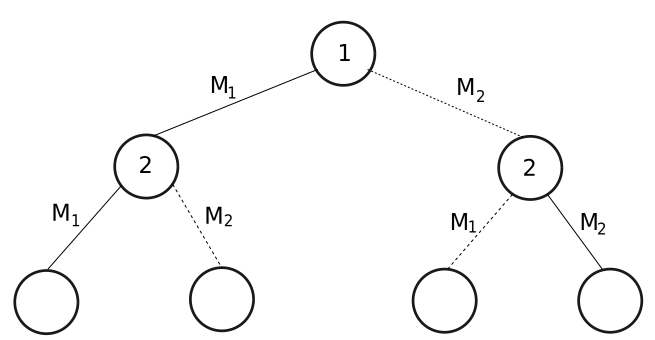
\includegraphics[scale=.3]{structural}
	\caption{Conflicting configuration}
	\label{fig:conflicting}
\end{figure}


\subsection{Linear lower bound}
Extending  the construction for $n=5$ players is non trivial as this seems to require rather involved constants that multiply the $\epsilon$ terms. However, we notice that these terms only help to induce more involved tie breaking rules of the following form:


\begin{definition}[arbitrary tie breaking rule]
	We say that the tie breaking rule is arbitrary if each player uses a tie breaking rule between machines which possibly depends on the strategies played by the previous players in the tree.
\end{definition}

%\begin{assumption}
%	Each player uses a tie breaking rule between machines which possibly depends on the strategies played by the previous players in the tree.  %\pp{This is not wlog, right? See \Cref{rem:tie-breaking}}
%\end{assumption}

The following theorem gives a general result:

\begin{theorem}
\label{counterexample}
Even for two machines, the \SPoA is at least linear in the number $n$ of jobs, in the case of arbitrary tie breaking rule.
%The sequential price of anarchy for $2$ machines is at least linear in the number of jobs $n$. 
\end{theorem}

\begin{proof}
We consider the following instance with $n=3k-1$ jobs arriving in this order
%weights on the first machine to be equal to $(k+1,0,0,k,0,0,\cdots, 3,0,0, 1, 2)$, job weights on the second machine to be equal to $(0,k-1,k-1,0,k-2,k-2,\cdots, 0,2,2, 1, 1)$. 
%
\[\begin{array}{c||c|c|c|c|c|c|c|c|c|c|c|c|}
& J_1 & J_2 & J_3 & J_4 & J_5 & J_6 &  & J_{3k-5} & J_{3k-4} & J_{3k-3} & J_{3k-2} & J_{3k-1} \\ \hline\hline
M_1 & \take{k+1} & 0 & \take{0} & k & \take{0} & \take{0} & \cdots & 3 & \take{0} & \take{0} & 1 & 2 \\ \hline
M_2 & 0 & \take{k} & k & \take{0} & k-1 & k-1 &  & \take{0} & 2 & 2 & \take{1} &  \take{1} \\ \hline
\end{array}
\]
and prove that the subgame perfect equilibrium is the gray allocation which results in a makespan $k+2$, while the optimal makespan is $1$. This requires players to use the following tie breaking rules in the first part: if player $J_1$ chooses machine $M_1$, then $J_2$ and $J_3$ prefer to avoid player $J_1$, that is, they choose the other machine in case of ties in their final cost. 


We prove this by induction on $k$. The base case is $k=2$ and it follows directly from the example in \Cref{eq:SPE:five-players} with $\epsilon=0$. As for the inductive step, the proof consists of the following two steps (claims below).
%\begin{enumerate}
%	\item If the first three jobs $J_1,J_2$ and $J_3$ choose the machine whose processing time is $0$, then the remaining jobs $J_4,\ldots,J_{3k+2}$ implement the subgame perfect equilibrium that would result from the same sequence above with $k'=k-1$.
%	\item If $J_1$ chooses the machine with processing time $0$, then both $J_2$ and $J_3$ will choose the machine with processing time $0$.
%\end{enumerate}

\begin{claim}
	If the first three jobs choose their zero-cost machines, then all subsequent jobs implement the subgame perfect equilibrium on the same instance with $k'=k-1$. The cost of $J_1$ in this case is $k'+2=k+1$.
\end{claim}
\begin{proof}[Proof of Claim]
	Note that the sequence starting from $J_4$ is the same sequence for $k' =k-1$. Since the first three jobs did not put any cost on the machines, we can apply the inductive hypothesis and assume that all subsequent players play the subgame perfect equilibrium. The resulting cost on machine $M_2$ will be $k'+2=k+1$, and this is the machine chosen by $J_1$.
\end{proof}

\begin{claim}
	If the first job $J_1$ chooses $M_2$, then both $J_2$ and $J_3$ choose $M_1$.
\end{claim}
\begin{proof}[Proof of Claim] 
	Choosing $M_2$ costs $J_2$ and $J_3$ at least $k$, no matter what the subsequent players do. If they instead choose $M_1$, by the previous claim, their cost is $k'+1=k$ which they both prefer given their tie breaking rule.
\end{proof}

%
%If $J_1$ chooses $M_1$ then her cost will be at least $k+1$ just because of its own cost on this machine. Therefore, by assuming $J_1$ breaks ties in favor of $M_2$, we have that 
%
%
%\pp{This last of the proof part should be adapted to the previous one}

The above two claims show that if $J_1$ chooses machine $M_2$ then she is paying a cost $k+1$, while in the following we show that if she chooses machine $M_1$, she will pay a cost $k+1$ in this scenario as well. The tie-breaking rule is that player $J_1$ prefers the cost $k+1$ on the first machine $M_1$.

In the second part of the proof we assume different tie-breaking rules for the last two players $J_{3\cdot k - 2}$ and $J_{3\cdot k - 1}$, depending on which of the two players $J_2$ and $J_3$ choose machine $M_2$.

Now we consider the case where job $J_1$ chooses machine $M_1$, and show that she pays exactly $k+1$.  If player $J_2$  chooses machine $M_1$, then we assume that  player $J_3$ breaks ties in favor of $M_2$: choosing  $M_2$ results in a cost of $k+1$ in the end, instead of some cost on machine $M_1$, which is at least $k+1$. If job $J_3$ gets assigned to machine $M_2$ then by backwards induction we can show that no player among $J_4,\cdots, J_{3\cdot k-3}$ gets assigned to machine where they have non-zero cost. This way only the last two players are left and we can assume that player $J_{3\cdot k-2}$ prefers to get assigned to machine $M_1$ and pay $k+2$ instead of getting assigned  to machine $M_2$ and pay $k+2$ there, while the last player $J_{3\cdot k-1}$ prefers to get assigned to machine $M_2$ and pay the cost $k+1$ there. Therefore, job $J_2$ gets cost $k+2$, but here we can assume that she prefers cost $k+2$ that she gets on machine $M_2$. Therefore, job $J_2$  gets assigned to machine $M_2$ in the subgame perfect equilibrium state. Then again, by the same backwards induction we conclude that all players $J_3,\cdots, J_{3\cdot k-3}$ get assigned to the machine where they have cost $0$, and the last two jobs $J_{3\cdot k-2}$ and $J_{3\cdot k-1}$ choose machine $M_2$, here again we assume that player $J_{3\cdot k-2}$ prefers to pay $k+2$ on machine $M_2$ than to pay the same cost on machine $M_1$. This way the load on machine $M_1$ is $k+1$, while the load on machine $M_2$ is $k+2$, which finishes the proof of the theorem.  

\end{proof}

\begin{remark}\label{rem:tie-breaking}
It is worth noting that in \cite{SPOAcongestion} authors consider a different game (routing) and construct an unbounded lower bound example for the sequential price of anarchy, but their analysis heavily uses a carefully chosen tie-breaking rule. We solved linear programs with strict inequalities obtained from the subgame perfect equilibria tree structure given in the example from the above proof. There are solutions for $n=8$ and $n=11$, that is linear programs are feasible. Therefore, at least for small $n$'s we can drop the assumption about tie-breaking rules completely, but the solution involves complicated coefficients for $\epsilon$'s and for the sake of exposition we do not present the exact solutions here. %\pp{I'm not sure this is a proof: it is a strong indication only}
\end{remark}


\begin{remark}
We could not find any example that would give an (even locally) better lower bound on sequential price of anarchy than it is in the proof of \Cref{counterexample}. For $n\leq 7$, our computer program searched the whole space and the results obtained above are the best. We believe that the construction from the proof of the theorem gives the best lower bound example. 
\end{remark}

\section{Linear upper bound on the \SPoS}
\label{sec:linear_upper_bound}

In this section we give a \emph{linear upper bound} on the  sequential price of stability for two machines (\Cref{th:SPoS} below). Unlike in the case of the sequential price of anarchy, here we have the freedom to  choose the order of the players (and suggest a particular tie breaking rule). Though finding the best order can be difficult, we found that a large set of permutations already gives a linear upper bound on \SPoS. In particular, it is enough that the ``authority'' divides the players into \emph{two groups} and put players in the first group first, followed by the players from the second group. Inside each group players can form \emph{any order}. The main result of this section is the following theorem:

\begin{theorem}\label{th:SPoS}
For two machines, the \SPoS is at most $\frac{n}{2}+1$.
%The sequential price of stability is at most $\frac{n}{2}+1$ for $2$ machines. 
\end{theorem}

\begin{proof}
Consider an optimal assignment and denote the corresponding makespan by $OPT$. By renaming jobs and machines, we can assume without loss of generality that in this optimal assignment machine $M_1$ gets jobs the first $k\leq \frac{n}{2}$ jobs, and machine $M_2$ gets all the other jobs:
\begin{align*}
\{J_1,J_2,\ldots, J_k\} \rightarrow M_1 \enspace,  && \{J_{k+1}, \ldots, J_n\} \rightarrow M_2 \enspace .
\end{align*}
% That is, $J_1,J_2,\ldots, J_k$ are assigned to $M_1$,  while machine $M_2$ gets all other jobs, $J_{k+1}, \ldots, J_n$.  
Take the sequence given by the jobs allocated to $M_1$ followed by the jobs allocated to $M_2$, 
$$J_1, J_2, \ldots, J_k, J_{k+1},\ldots, J_n.$$ We prove that for this sequence there is a subgame perfect equilibrium whose makespan is at most $(k+1)\cdot OPT$. 

In the proof we consider the \emph{first player who deviates}. We distinguish two cases. 

\begin{claim}
	If the first player $J_d$ who deviates is in $\{J_{k+1}, \ldots, J_n\}$, then she does not improve. 
\end{claim}
\begin{proof}[of Claim]%% comment in LNCS [Proof of Claim] %%%
	Observe that all players in $\{J_1,J_2,\ldots, J_k\}$, that come before player $J_d$, did not deviate. Machine $M_1$ has all jobs that it gets in the optimum. If $J_d$ stays in $M_2$, her cost will be at most $OPT$. Moving to $M_1$ will in the end produce a feasible allocation with fewer jobs on $M_2$ and more jobs on $M_1$, compared to the optimum. The cost on $M_1$ is therefore at least $OPT$, which is the cost of $J_d$ when deviating.  
\end{proof}

The remaining  case is the following one.

\begin{claim}
	If the first player $J_d$ who deviates is in $\{J_{1}, \ldots, J_k\}$, then any subgame perfect equilibrium has the makespan at most $(t+1)\cdot OPT$ where $d=k+1-t$.
\end{claim} 
\begin{proof}[of Claim]%% comment in LNCS [Proof of Claim] %%%[Proof of Claim]
	The proof is by induction on $t$. For $t=1$, the deviating player is the last in $\{J_{1}, \ldots, J_k\}$. If the first deviating player is $J_k$, then the reason she deviated is because in the final solution she is paying at most $OPT$. We argue that in that case $M_1$ will have load at most  $2\cdot OPT$. This is because if no player among $J_{k+1},\ldots, J_n$ deviates to machine $M_1$, then the final load on this machine will be at most $OPT$. If any player deviated to $M_1$ this is because she is paying at most $2\cdot OPT$ in the final solution, otherwise she would stay on the second machine and pay at most $2\cdot OPT$.
	
	If the first player who deviates from the optimal assignment is $J_{k-t}$, then we argue similarly that the makespan is at most $(t+1) \cdot OPT$. By induction we can assume that if player $J_{k-t}$ stays on the first machine then she is guaranteed to pay at most $t\cdot OPT$, while if she deviates then we know she is paying at most $t\cdot OPT$ on the second machine. In the latter case, if any player $J_{k+1}, \ldots, J_{n}$ deviates from the second machine to the first machine then she is paying at most $(t+1) \cdot OPT$, because otherwise she would stay on the second machine and pay at most $(t+1) \cdot OPT$. Therefore, by induction we get that this sequence results into a solution which has a makespan at most $(k+1)\cdot OPT$, which completes the proof.
\end{proof}

%If this player is among $\{J_{k+1}, \ldots, J_n\}$, then the optimality of the allocation implies that this player does not improve: 
%\begin{enumerate}
%	\item All players in $\{J_1,J_2,\ldots, J_k\}$ did not deviate, and therefore are allocated to $M_1$.
%	\item If this player deviates, in the end she will join those that are in $M_1$ in the optimum, while $M_2$ will have less jobs. Since the original allocation was optimal, the cost on $M_1$ is at least $OPT$.
%\end{enumerate}
%
%The proof is by induction on the index of the first player who deviates from the optimum assignment. First we show a base case. It is impossible that this player is among $J_{k+1}, \ldots, J_n$, because it contradicts the optimality of this allocation (note that all other jobs $J_1,\ldots,J_k$ did not deviate and therefore choose $M_1$). If the first deviating player is $J_k$, then the reason she deviated is because in the final solution she is paying at most $OPT$. We argue that in that case $M_1$ will have load at most  $2\cdot OPT$. This is because if no player among $J_{k+1},\ldots, J_n$ deviates to machine $M_1$, then the final load on this machine will be at most $OPT$. If any player deviated on the $M_1$ this is because she is paying at most $2\cdot OPT$ in the final solution, otherwise she would stay on the second machine and pay at most $2\cdot OPT$. If the first player who deviates from the optimal assignment is $k-t$, then we argue similarly that the makespan is at most $(t+1) \cdot OPT$. By induction we can assume that if player $J_{k-t}$ stays on the first machine then she is guaranteed to pay at most $t\cdot OPT$, while if she deviates then we know she is paying at most $t\cdot OPT$ on the second machine. In the latter case, if any player $J_{k+1}, \ldots, J_{n}$ deviates from the second machine to the first machine then she is paying at most $(t+1) \cdot OPT$, because otherwise she would stay on the second machine and pay at most $(t+1) \cdot OPT$. Therefore, by induction we get that this sequence results into a solution which has a makespan at most $(k+1)\cdot OPT$, which completes the proof.

The two claims above imply the theorem\qed\end{proof}

\begin{remark} 
This result cannot be extended to more than $2$ machines, because the third machine would change the logic of the proof. We can no longer assume that players on the second machine in the optimum assignment can guarantee low costs for them just by staying on the second machine.
\end{remark}

\section{Achieving the optimum: the \aSPoS}
%\section{Optimum sequential scheduling}
\label{sec:optimum_sequence}

In this section we study the adaptive sequential price of stability. Unlike the previous models, here we assume that there is some authority who is very strong, meaning that it has a full power on the order of players. It cannot only fix the complete order, but can also change the order depending what decision previous players get. On the other hand players still have a complete freedom into choosing any strategy and therefore, the best outcome for them. We also assume that all players know the whole structure of a decision tree defined by the authority. This model is the closest instantiation of a general extensive form game compared to the previous models in this paper. This way the authority has an option to punish players for deviating from the optimum path by placing different players after the deviating player in case of different decisions. Therefore, rational players may achieve much better solutions in the end. The following theorem shows that achieving the optimum solution is possible for $2$ machines:




\begin{theorem}\label{optimum_sequence}
For two machines, the $\aSPoS$ is $1$.
%The \asPoS\ adaptive sequential price of stability is $1$ for $2$ machines.
\end{theorem}

\begin{figure}
	\centering
	\includegraphics[scale=.65]{find_next_player}
	\caption{Initial constrained optimum on left, new constrained optimum on right}
	\label{fig:next_player}
\end{figure}

\begin{proof}
The main idea of the proof is backwards induction. In each subtree of a decision tree we aim to implement constrained optimum. Under constrained optimum in each subtree we mean the optimum makespan solution that is possible to achieve by the remaining players in the subtree given the initial loads on both machines created by the players arriving before this point. The root of each subtree is chosen in the following way: choose the player who gets worse outcome in the case of a deviation from the optimum strategy. More formally, for each subtree  consider the constrained optimum solution, we prove that there is at least one player so that if this player is assigned to a different machine from that it is assigned in the constrained optimum, then in a new constrained optimum she gets a larger cost and therefore this deviation is undesirable for the player.  Using backwards induction we can assume that in each subtree new constrained optima are implemented. Therefore, if we show the claim then it finishes the whole proof of the theorem. The proof of the claim is the following: without loss of generality consider any player from machine $M_1$ and put it on the machine $M_2$, we know that in the new constrained optimum, the makespan is at least the same as the original makespan by definition, which means that either this player or some other player from the machine $M_2$ in the original constrained optimum assignment gets worse outcome. We choose the player who gets a worse (or the same) outcome and this finishes the proof of the claim. See \Cref{fig:next_player} for the illustration. 
\end{proof}

Unfortunately, this result cannot be extended to more than $2$ machines. We show this in the following theorem:

\begin{theorem}
For three or more machines, the \aSPoS is at least $\frac{3}{2}$.
\end{theorem}

\begin{proof}
%Proof by example: suppose $n=m=3$ and the processing times on the machines are the following vectors $(6,6-\epsilon,6-\epsilon)$, $(4-\epsilon, 2,2)$ and $(4, 3,3)$. 
%
Consider the following instance with three machines and three jobs, where the optimum is shown as gray boxes:
\begin{align*}\begin{array}{c||c|c|c|}
& J_1 & J_2 & J_3 \\ \hline \hline
M_1 & 4 -\epsilon &  \take{2} & \take{2}  \\ \hline
M_2 & \take{4} & 3 & 3  \\ \hline
M_3 & 6 & 6-\epsilon & 6-\epsilon  \\ \hline 
\end{array} &&
\end{align*}
Note that $M_1$ is the cheapest machine for each job, $M_2$ is the second-cheapest, and $M_3$ is the most expensive one. We claim that, for any adaptive sequence (tree), the resulting subgame perfect equilibrium will have the following structure:
\begin{itemize}
	\item The first job \emph{to move} will choose $M_1$, the second one $M_2$, and the third one $M_3$. 
\end{itemize}
%\begin{align*}\begin{array}{c||c|c|c|}
%& J_1 & J_2 & J_3 \\ \hline \hline
%M_1 & 6 & 6-\epsilon & 6-\epsilon  \\ \hline 
%M_2 & 4 -\epsilon &  \take{2} & \take{2}  \\ \hline
%M_3 & \take{4} & 3 & 3  \\ \hline
%\end{array} &&
%\end{align*}
This implies that the cost is at least $6-\epsilon$, and thus the lower bound holds by taking $\epsilon$ small enough. 
To prove the claim above, we observe the following. Suppose the first two jobs to move choose $M_1$ and $M_2$. Then, the third job will choose $M_3$ as  in some  among the first two jobs chooses $M_3$ (otherwise we are done). Assume the third job will always choose the machine left empty. Then, for the second job it is always better to not join the same machine of the first one
%Assuming the first wo jobs have chosen different machines. While the optimum is $4$, we claim that any adaptive sequence (tree) will have subgame perfect equilibrium with makespan at least $6 - \epsilon$. Note that $J_2$ and $J_3$ have the same costs, and therefore there are only the following cases to consider:
%\begin{enumerate}
%	\item The first is $J_1$. If $J_1$ goes to $M_2$, none of the other two jobs will join this machine as they will go one on $M_1$ and one on $M_3$. 
%	\item The first is $J_2$. If $J_2$ goes to $M_2$, the next job will not join this machine and rather choose the cheapest of the remaining two. 
%\end{enumerate}
%
%It is easy to note that the optimum makespan is $4$, while by trying all adaptive sequences we get that the makespan is at least $6-\epsilon$. Obviously, we can always add dummy machines (and players) to generalize this result to more machines (and more players). 
\end{proof}

\begin{remark}
The analysis in the proof of \Cref{optimum_sequence} cannot be extended to more than $2$ machines even if we assume that the machines are identical. The following example shows this. Assume that we have $m=3$ machines, the initial loads on these machines are $(0,2,6)$ and there are $3$ jobs left to be assigned with processing times $7, 5$ and $5$. Note that the constrained optimum here is $(10, 9, 6)$, that is the first job with processing time $7$ gets assigned to the second machine $M_2$, while both jobs with processing times $5$ and $5$ get assigned to machine $M_1$. On the other hand, if any of these players chooses different machine their cost is strictly decreasing in the subgame perfect equilibrium solution. We did not find any example where the claim of \Cref{optimum_sequence} is wrong for more than $2$ identical machines, unlike the case of unrelated machines.      
\end{remark}




\section{Conclusions}\label{sec:conclusion}

In this paper we disproved a conjecture from \cite{Hassin} and gave a linear lower bound construction. On the other hand, for the best sequence of players we proved a linear upper bound, moreover we proved an existense of a sequential extensive game which gives an optimum solution. One possible direction for a future research is to prove or disprove that sequential price of stability is $1$ for identical machines. Up to this point, we were unable to prove it or find a counterexample. 


\paragraph{Acknowledgments.} We thank Paul D\"{u}tting for valuable discussions. 


% \bibliographystyle{plainnat}
\bibliographystyle{plain}
\bibliography{sequential}

\end{document}